\section*{Assignment 2: Transmission Lines in Time Domain}
\addcontentsline{toc}{section}{\protect\numberline{}Assignment 2: Transmission Lines in Time Domain}

\subsection*{Part 1: Time Domain Reflectometry: estimate the load’s impedance}

\begin{figure}[h!]
\centering
\includegraphics[width=\textwidth]{plots/ZL.eps}
\caption{Recording with ZL as load}
\label{fig:ZL}
\end{figure}

As seen in Figure \ref{fig:ZL}, the incident signal ranges from around -30 to 120 mV and the reflected signal -30 to 0 mV. \\
By increasing the values by 30, the values of $E_i \approx 150mV$ and $E_r \approx 30mV$ can be found. 
\begin{equation}
\Gamma = E_r/E_i = 0.2
\end{equation} 

$Z_l$ can be determined with equation \ref{zload} with $Z_0 = 50 \Omega$

\begin{equation}
\label{zload}
	\Gamma = \frac{Z_l-Z_0}{Z_l+Z_0}
\end{equation}

\begin{equation}
	Z_l = - \frac{\rho + 1}{\rho - 1} \cdot Z_0 = 75 \Omega
\end{equation}

\subsection*{Part 2:  Dielectric in Coaxial Cable: the Estimation of the Propagation Speed and Relative Permittivity}

\begin{figure}[h!]
\centering
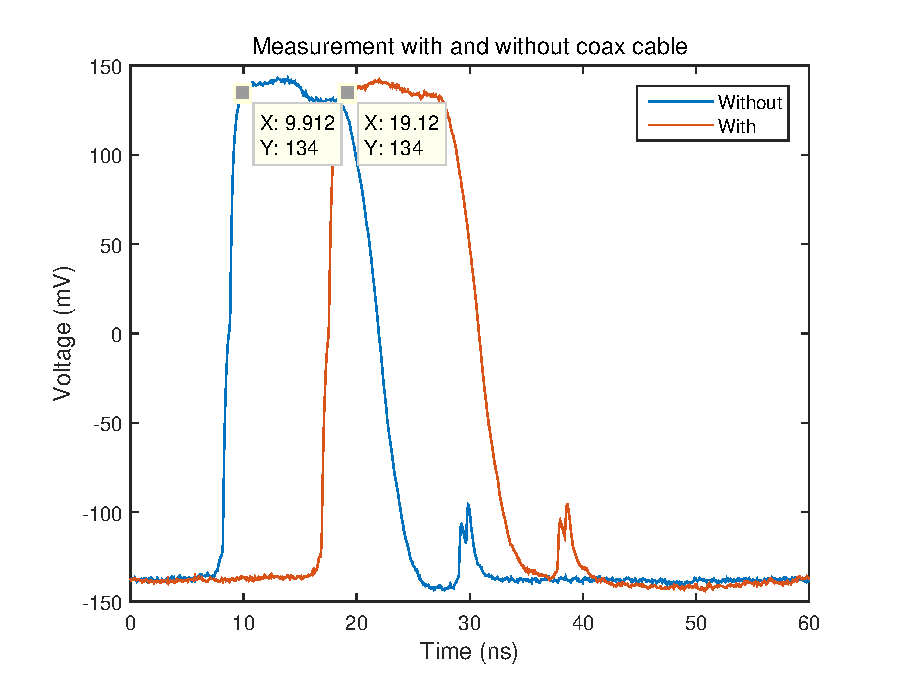
\includegraphics[width=\textwidth]{plots/part_2.eps}
\caption{Recording with and without coaxial cable}
\label{fig:p2}
\end{figure}

By measuring the time the signal is delayed after the 2 meter long coaxial cable is connected, the propagation velocity can be calculated. As seen in Figure \ref{fig:p2}, the time difference is 9.2 ns. The propagation velocity can now be calculated:

\begin{equation}
	v = s/t = 2.17*10^8 m/s = 0.72*c
\end{equation}

From the reflections the propagation velocity turned out to be $0.72c$, which is slightly less than the 0.77c, stated by the datasheet of the cable \cite{datasheetcable}. 
Using equation \ref{propvel} the relative permittivity $\epsilon_r$ can be calculated.

\begin{equation}
\label{propvel}
	v = \frac{c}{\sqrt{\epsilon_r}} = 0.72 c
\end{equation}

\begin{equation}
	\epsilon_r = (\frac{c}{v})^2 = 1.91
\end{equation}
